\chapter{Preliminaries}
\label{chap:prelims}
As a preliminary discussion to the presentation of our contribution, we overview some the key theoretical basis of the thesis.
First, a short overview of array-processing is presented in Sec.~\ref{sec:prlm_sensorArrays}, accompanied by a complementary wave propagation discussion in Sec.~\ref{sec:prlm_propWaveField}.
To accommodate the discussion for spatial filtering, we also mention the time-space relation of spatially sampled signals in Sec.~\ref{sec:prlm_timeSpaceSig}.
In Sec.~\ref{sec:prlm_localization}, we further focus the spatial filtering discussion to localization and overview some of its fundamentals.
Following the FIR/IIR filters related issue, which was previously mentioned in Chapter.~\ref{chap:intro}, we further elaborate and compare the two architectures in Sec.~\ref{sec:prlm_FIR_IIR}.
To complete the basics overview, we also discuss array performance measures in Sec.~\ref{sec:prlm_array_perf} following classical array processing literature.
% \begin{definition}
% The \emph{von Neumann model} of a computer, also known as the \emph{Princeton architecture} is an architecture for digital computers, which consists of a processing units, containing an ALU and processing registers; a control unit consisting of an instruction register and a program counter; a memory unit which stores both data and instructions; and input-and-output mechanisms.
% \end{definition}

% \section{Digital Filter Design - Finite/Infinite Response Filters}
% \label{sec:prlm_FILTERS}
% A basic building block of any signal processing system is the digital filter, which manipulates input signals according to some predetermined specifications. 
Nominally, digital filters are applied to temporal-domain sampled signals, while designed to meet certain frequency-domain specification.
The most  
\section{Sensor arrays}
\label{sec:prlm_sensorArrays}
Microphone arrays consist of sets of microphones positioned in a way to function as a directional acoustic antenna. 
Microphone arrays are utilized for filtering signals in a space-time field. 
Filtering is enabled by exploitation of the incoming signals spatial characteristics. 
A desirable spatial filtering, i.e., beamforming, should result in enhancement of signals of interest, originated in a specific direction, while forcing suppression of undesired signals originated in other directions.
Microphone arrays are utilized for solving many signal processing problems: dereverberation, localization of a single source, noise reduction and source separation \cite{cohen2004multichannel,habets2006dual,pavlidi2013real}.
\par 
Numerous factors must be taken into consideration when designing a microphone array configuration.
Initially, the geometry of the microphone array plays an important role in the formulation of the processing algorithms, as it forces fundamental constraints on the array’s operation. 
In most cases, the array geometry is the first consideration in array design due to practical and physical constraints of the design. 
Therefore, the degree of freedom in choosing the array geometry is limited. 
Nevertheless, in some other crucial problems such as noise reduction or source separation, the geometry of the array may have little importance. 
For instance, Uniform Linear Arrays (ULA) can only handle one source direction at a time resulting in uncertainties and possibly direction ambiguities.
Therefore, ULA configurations must be ruled out when handling several signal sources.
Other array geometries such as non-uniform linear arrays and circular arrays, have been studied in the field \cite{liu2008design,van2004optimum}.
This work is based on ULA and therefore we elaborate on this geometry.
A conventional beamformer \cite{van2004optimum} is composed of a ULA of microphones. 
That is, the microphones are positioned on an axis with a uniform spacing between the microphones.
The general expression of the microphone positioning in a ULA is given by:
\begin{equation}
x_{m}=m\cdot{d}, m=0, 1, \dots, M-1
\end{equation}
where $m$ denotes the microphone index; $x_{m}$ denotes the position of the microphone having index $m$, where $x_{m} = 0$ corresponds to the left-hand side of the array, i.e., the location where the microphone indexed by $m = 0$ is positioned; $d$ denotes the spacing between microphones, and $M$ is the array size, i.e., the number of microphones in the array, as demonstrated in Fig.~\ref{fig_ULA}.
\begin{figure}[h!]
    \begin{center}
        \begin{overpic}[width=0.5\linewidth, 
        %grid, 
        tics=10,trim=0 0 0 0]{./Media/fig_ULA.png}
            % \put (50, 62.5) {\footnotesize{$r=0$}}
        \end{overpic}
    \end{center}
     \caption{A uniform linear array of size M and spacing d.}
    \label{fig_ULA}
\end{figure}
\section{Propagating Wave Fields}
\label{sec:prlm_propWaveField}
% In array signal processing, propagating waves carry signals from the source to the array.
% Therefore, these signals are represented in the time-space domain. The space domain is represented by either the three dimensional Cartesian coordinates $\rBrace{x,y,z}$ or the three dimensional spherical coordinates $\rBrace{r,\phi,\theta}$, where $0 \leq \phi \leq 2\pi$, $0 \leq \theta \leq \pi$ are the azimuth and elevation angles, respectively. The time domain is represented by $t$.
An elementary physical phenomenon is the spatial dynamics of waves, referred to as wave-propagation.
The spatial location is noted by the Cartesian coordinates $\rBrace{x,y,z}$ or the three dimensional spherical coordinates $\rBrace{r,\phi,\theta}$, where $0 \leq \phi \leq 2\pi$, $0 \leq \theta \leq \pi$ are the azimuth and elevation angles, respectively. 
% Finally, let $f\rBrace{t,\vecnot{r}}$ denote the time-space representation of the input signal, where $\vecnot{r}$ is the radius-vector in the three-dimensional system. 
% The relations between the Cartesian and spherical coordinates are given in Fig.~\ref{fig_coordinates}.
Denoting $t$ as the time, the time-space representation of the a signal is $f\rBrace{t,\vecnot{r}}$ or , where the relations between the Cartesian and spherical coordinates are given in Fig.~\ref{fig_coordinates}.
% $f\rBrace{t,x,y,z}$ describes the signal impinging the microphone array. 
In a homogeneous, dispersion free and lossless medium the wave equation is:
\begin{equation}
\label{eq_prlm_waveEq}
\nabla^{2}f\rBrace{t,x,y,z}=\frac{1}{c^2}\frac{\partial^{2}f\rBrace{t,x,y,z}}{\partial{t^{2}}}
\end{equation}
where $\nabla^{2}$ is the Laplacian operator and $c$ represents the wave's velocity in the medium.
\begin{figure}[h!]
    \begin{center}
        \begin{overpic}[width=0.5\linewidth, 
        %grid, 
        tics=10,trim=0 0 0 0]{./Media/fig_coordinates.png}
            % \put (50, 62.5) {\footnotesize{$r=0$}}
        \end{overpic}
    \end{center}
     \caption{A three dimensional coordinate system with Cartesian and spherical coordinates.}
    \label{fig_coordinates}
\end{figure}
A possible solution to \eqref{eq_prlm_waveEq}, $f_p\rBrace{t,x,y,z}$, may be of a complex exponential form:
\begin{equation}
\label{eq_prlm_waveEq_pSol}
f_p\rBrace{t,x,y,z} = A\exp{j\rBrace{\omega{t}-k_{x}x-k_{y}y-k_{z}z}}
\end{equation}
Where $A$ is a complex constant, $\omega$ denotes temporal radial frequency and $k_{x}x,k_{y},k_{z}$ are real constants. 
Plugging \eqref{eq_prlm_waveEq_pSol} into \eqref{eq_prlm_waveEq} results in the \emph{monochromatic plane wave}:
\begin{equation}
\label{eq_prlm_waveEq_subs}
k_{x}^{2}-k_{y}^{2}-k_{z}^{2} = \frac{\omega^{2}}{c^{2}}.
\end{equation}
Using the plane wave notation emphasizes the fact that for a given time, $t_{0}$, all points on a plane given by $k_{x}x+k_{y}y+k_{z}z = constant$ are with the same wave value and the vector notation of \eqref{eq_prlm_waveEq}'s solution is
\begin{equation}
\label{eq_prlm_waveEq_finSol}
f\rBrace{t,\vecnot{x}}=A\exp{j\rBrace{\omega{t}-\vecnot{k}\vecnot{x}}}.
\end{equation}
where $\vecnot{k}\vecnot{x}=constant$ are planes of constant wave value.
The wave propagation can be described as the traveling of the planes, stating that small steps of both space $\delta{\vecnot{x}}$ and time $\delta{t}$ result in the same wave value i.e. $f\rBrace{t+\delta{t},\vecnot{x}+\delta{\vecnot{x}}} = f\rBrace{t,\vecnot{x}}$, which yields
\begin{equation}
\omega\delta{t}-\vecnot{k}\delta\vecnot{x}=0.
\end{equation}
Assuming $\delta\vecnot{x}$ and $\vecnot{k}$ have the same direction, $\vecnot{k}\delta\vecnot{x} = \abs{\vecnot{k}}\abs{\delta\vecnot{x}}$ and $\frac{\delta{\vecnot{x}}}{\delta{t}} = \frac{\omega}{\abs{\vecnot{k}}}$, where $\frac{\delta{\vecnot{x}}}{\delta{t}}$ can designate the propagation speed of the plane wave. 
Since $\vecnot{k}$ and $\omega$ are related by $\abs{\vecnot{k}}^{2}=\frac{\omega^{2}}{c^{2}}$, we have
\begin{equation}
\label{eq_prlm_waveEq_stepsEq}
\frac{\delta{\vecnot{x}}}{\delta{t}}=c,
\end{equation}
where $c>0$ is the wave velocity in the medium.
The \emph{wavelength} ($\lambda$) denote the distance the plane wave propagated during a single temporal period of $T=\frac{2\pi}{\omega}$.
Let $\vecnot{k}$ denote the \emph{wavelength vector}. 
Its magnitude $\abs{\vecnot{k}}$ expresses the number of cycles in radians per meter of length that the plane wave has exhibited in the propagation direction.
Using \eqref{eq_prlm_waveEq_stepsEq} with $\delta{t} = \frac{2\pi}{\omega}$, we obtain:
\begin{equation}
\lambda=\delta{\vecnot{x}}=\frac{2\pi}{\abs{\vecnot{k}}}.
\end{equation}
Therefore, the wavenumber vector can be considered to represent spatial frequency, similarly to the manner $\omega$ represents temporal frequency.
\par For example, in the context of ULA, assuming far field scenario, the impinging waves are treated as constant phase planes as in \eqref{eq_prlm_waveEq_finSol}.
The spatial diversity of the ULA elements is expressed as a TOA difference of the impinging signal in each sensor which is will be shown to provide clues for the signal's DOA as can be seen in Fig.~\ref{fig_ULA_sketch}.
\begin{figure}[h!]
    \begin{center}
        \begin{overpic}[width=0.6\linewidth, 
        %grid, 
        tics=10,trim=0 0 0 0]{./Media/arraySketch.png}
        \put(20,45){\rotatebox{-50}{\tiny{Impinging wavefront}}}
        \put(33.25,2.25){\rotatebox{0}{\tiny{$d$}}}
        \put(52.25,26){\rotatebox{38}{\tiny{$c\tau=d\cos{\theta}$}}}
        \put(49,15.75){\rotatebox{0}{$\theta$}}
        \put(15,7){\rotatebox{0}{\tiny{0}}}
        \put(28,7){\rotatebox{0}{\tiny{1}}}
        \put(41,7){\rotatebox{0}{\tiny{2}}}
        \put(80,7){\rotatebox{0}{\tiny{$N-1$}}}
        \put(44,36){\rotatebox{38}{\tiny{$t=\rBrace{N-1}\tau$}}}
        \put(57,36){\rotatebox{38}{\tiny{$t=\rBrace{N-2}\tau$}}}
        \put(70,36){\rotatebox{38}{\tiny{$t=\rBrace{N-3}\tau$}}}
        \put(92,25){\rotatebox{38}{\tiny{$t=0$}}}
        \end{overpic}
    \end{center}
     \caption{An illustration of an $N$ element ULA, impinged with a plane wave arriving from a DOA of $\theta$.}
    \label{fig_ULA_sketch}
\end{figure}
When also considering the narrowband scenario, where TOA difference is merely phase shift, it seems obvious that by phase measuring, one should be able to extract the DOA from the spatially sampled data.
\section{Spatio-temporal processing}
\label{sec:prlm_timeSpaceSig}
The incoming signals are spatially sampled by the array microphones, then the samples are processed to attenuate signals from undesired directions and extract the signal from a desired direction. 
A spatial response of the microphone array is obtained via a beam (main-lobe) directed to the desired signal while nulls are directed to the undesired signals.
\begin{figure}[ht!]
    \begin{center}
        \begin{overpic}[width=0.5\linewidth, 
        %grid, 
        tics=10,trim=0 0 0 0]{./Media/fig_ULA_imping.png}
            % \put (50, 62.5) {\footnotesize{$r=0$}}
        \end{overpic}
    \end{center}
     \caption{A simple beamformer design.}
    \label{fig_ULA_imping}
\end{figure}
Fig.~\ref{fig_ULA_imping} illustrates a beamformer design based on a ULA of Fig.~\ref{fig_ULA}.
Let $\vecnot{f}\rBrace{t,\vecnot{x}}$ denote the set of signals sampled by the microphone array at time $t$, expressed by
\begin{equation}
\vecnot{f}\rBrace{t,\vecnot{x}} = \vBrace{f\rBrace{t,x_{0}},\dots,f\rBrace{t,x_{M-1}}}^{T},
\end{equation}
where $x_{m}$ denotes the microphone position, $t$ denotes the continuous-time variable and $^{T}$ denotes the transpose operation. 
The beamformer output $y\rBrace{t}$ is expressed by:
\begin{equation}
y\rBrace{t} = \sum_{m=0}^{M-1}{f\rBrace{t,x_{m}}\omega_{m}^{*}},
\end{equation}
where $\omega_{m}$ is a complex weight of the microphone having index $m$, as shown in Fig.~\ref{fig_ULA_imping} and $^{*}$ denotes complex conjugation. 
The simplest beamformer design architecture has uniform weights, $\omega_{m}=\frac{1}{M}, m=0,\dots,M-1$.
Let $f_{\omega}\rBrace{t,x} = e^{j\omega{t}}$ denote a plane wave propagating at angular frequency $\omega$, and let $\theta \in \vBrace{-\frac{\pi}{2},\frac{\pi}{2}}$ denote the direction of arrival (DOA) angle measured with respect to the broadside of the linear array, as shown in Fig.~\ref{fig_ULA_imping}.
The wave signals spatially sampled by the microphone array inputs are given by:
\begin{equation}
\label{eq_prlm_timeSpace_outputVec}
\vecnot{f}\rBrace{t,x} = \vBrace{f_{\omega}\rBrace{t-\tau_{0}}, \dots, f_{\omega}\rBrace{t-\tau_{M-1}}}^{T}, \tau_{m} = \frac{\sin{\theta}\cdot{}x_{m}}{c},
\end{equation}
where $\tau_{m}$ is the propagation delay for the incoming signal and $c$ is the wave's velocity in the medium.
A value of $\tau_{m}=0, \forall{m}$ implies a DOA of $\theta = 0$, i.e. a plane wave parallel to the array, propagating perpendicularly to the array.
Let $\kappa=\frac{\omega}{c}\sin{\theta}=\frac{2\pi}{\lambda}\sin{\theta}$ denote the wavenumber for plane waves in a locally homogeneous medium, where λ denotes the wavelength corresponding to the angular frequency $\vecnot{v}\rBrace{\kappa}$ denote the \emph{array manifold vector} \cite{van2004optimum}, featuring all of the spatial characteristics of the microphone array.
Based on \eqref{eq_prlm_timeSpace_outputVec}, and the definition of κ above, the manifold vector can be expressed as
\begin{equation}
\vecnot{v}\rBrace{\kappa}=\vBrace{e^{-j\kappa{}x_{0}},\dots,e^{-j\kappa{}x_{M-1}}}^{T}.
\end{equation}
\section{Localization}
\label{sec:prlm_localization}
In the wide and very active research field of parametric estimation, one subject of very high relevance to this thesis is the sensor-array based localization - i.e. positional parameters estimation of impinging signal which is measured by an array of sensors.
In this work, we focus on localization of signal sources in the far-field case, where free space signal propagation is assumed.
Following the classical methods overview in \cite{krim1996two},most localization estimators may be divided to two main groups - i.e. \textit{spectral-based} and \textit{parametric}.
The basic difference between the two groups is the assumption of impinging signal's statistical model when using parametric approach, which leads to higher accuracy in the expense of computation effort.
In both approaches, the estimations are based on calculation of several hypothesis and choosing the peaks in the generated graph.
Considering the search for a single parameter (e.g. DOA in a 2D plane), the two approaches are pretty similar in the sense that in both, the processor computes the confidence in a predetermined set of hypothesis which is followed by a single dimension scan.
The difference is more evident when considering multiple parameter, such as spherical direction (i.e. azimuth and elevation) or even actual location adding also the distance to the target of interest.
In the spectral based, each parameter is estimated independently of the other parameters, resulting in several 1D scans (as the number of estimated parameters), where the parametric approach will result in a multi-dimensional search for the best fitted parameters set.
In the following, a basic overview of some classical algorithms is presented.
The earliest localization algorithms, which date back to world war II, are the beamforming based, e.g. the conventional Bartlet beamformer.
These methods, although appealing in terms of complexity and computation effort, suffer from fundamental limitation, e.g. its spatial performance depend solely on the array aperture and no improvement is achieved when more data is collected.
Another class of estimators, where a statistical model is assumed (which is also the drawback of those methods), is the parametric estimators such as Maximum-Likelihood \cite{TWODECADES-81/106} and Maximum-Entropy \cite{TWODECADES-23}.
Until the mid- 1970's, direction finding techniques required knowledge of the array directional sensitivity pattern in analytical form, and the task of the antenna designer was to build an array of antennas with a prespecified sensitivity pattern.
Trying to relax the need for such accuracy, also serving as the origin of the sub-space based approach, was the Multiple SIgnal Classification (MUSIC) \cite{MUSIC_} algorithm.
In general, the MUSIC algorithm consists of several stages:
\begin{itemize}
    \item Estimation of the covariance matrix
    \item Eigen decomposition - extracting the eigen values and its related eigen-vectors
    \item Estimating the number of sources
    \item Projecting the samples over the array manifold
    \item Finding the largest peaks according to the estimated number of sources
\end{itemize}
MUSIC essentially relieved the designer from the need of accurate radiation patterns by exploiting the reduction in analytical complexity that could be achieved by calibrating the array.
Thus, the array response calculation task was reduced to that of measuring and storing the response. 
Although MUSIC did not mitigate the computational complexity of solution to the DOA estimation problem, it did extend the applicability of high-resolution DOA estimation to arbitrary arrays of sensors.
Another, probably even more important breakthrough, was the introduction of the array manifold and noise space (hence its name - sub-space) which proved to be orthogonal, thus allowing the use of orthogonal projection.
In the very thorough review of classical algorithms \cite{TWODECADES}, two approaches - i.e. the parametric approach and ULA-specific algorithms are also discussed.
the parametric approach, where stochastic model is assumed and Maximum Likelihood (ML) and Stochastic Maximum Likelihood (SML) are employed, is less relevant to this work therefore not discussed.
In the set of ULA-specific algorithms, including ROOT-MUSIC \cite{ROOT_MUSIC}, ESPRIT (Estimation of Signal Parameters via Rotational Invariance Techniques) \cite{ESPRIT} and some iterative methods.
We choose to emphasize on the ESPRIT method, being an important milestone in the path to state-of-the-art algorithms.
In addition to using the rotational invariance of the signal sub-space eigenvectors, it also reduced computation and storage costs (especially in the multi-dimensional estimation case) by replacing the covariance matrix calculation and eigendecomposition by a relaxed partial singular value decomposition (SVD) which is employed on the data itself without squaring it - mitigating numerical problems associated with ill-conditioned matrices.
Following state-of-the-art developments \cite{BOOK-classicalAndModernDOA}, the sub-space based algorithms are still modified and adjusted to specific scenarios as in \cite{LpNorm MUSIC} but also new and interesting approaches emerged
\begin{itemize}
    \item High Order Statistics (HOS, also refereed as comulants), which extracts more information from the samples' higher order moments, is a very active field of research due to some fundamental issues which are inherently resolved - i.e. the Gaussian noise vanishes in the 4th order statistics and the ability to resolve more DOAs than array elements.
    This approach, being costly in computation effort, became popular probably due to the recently available low-cost powerful computation.
    \item Sparsity based estimation, using non-Frobenius norm used in the algorithms development, has proved to improve estimation resolution in some cases \cite{LocalizationOfMultipleSpeaker}, namely high reverbrant acoustic scenarios, but is less relevant to this work therefore not elaborated.
    \item A very wide and active research field is the concept of cooperative localization related to mobile networks is growing at a very high rate due to the never-ending need for high-bandwidth and low-power communication of the mobile networks.
    It is also less relevant to this work.
    \item Naturally, also many trials of harnessing the promising concept of neural networks are being done, for example \cite{NNDOA}
\end{itemize}
In this work, we actually revisit the most basic approach - i.e. beamforming.
% \section{Sensor array performance measure}
% \label{sec:prlm_sensorArrayPerf}
% Numerous performance measures are utilized for evaluating the microphone array capabilities. 
Each of the measures aims to quantify a significant aspect of either the response of an array to the signal environment or of the sensitivity to an array design error.
First, we review the concept of beampatterns. 
Beampatterns are the main tool in assessing an array performance as they express the beamformer response for various frequencies and signal angles. 
Let $P\rBrace{\omega,\theta}$ denote the frequency and DOA dependent beamformer response. It is given by:
\begin{equation}
P\rBrace{\omega,\theta}=\sum_{m=0}^{M-1}e^{-j\omega\tau_{m}w_{m}^{*}}=\vecnot{w}^{H}\vecnot{v}\rBrace{\omega,\theta}    
\end{equation}
where $\vecnot{w}=\vBrace{w_{0},\dots,w_{M-1}}^{T}$ and $^{H}$ denotes Hermitian transpose operation, and let $D\rBrace{\omega,\theta}$ denote the beampattern of a given beamformer. 
It is expressed by:
\begin{equation}
D\rBrace{\omega,\theta}=20\log_{10}\abs{P\rBrace{\omega,\theta}},
\end{equation}
where $\abs{\cdot}$ denotes the absolute value. 
For a given angular frequency $\omega$, the beampattern $D\rBrace{\omega,\theta}$ is a function of the angle $\theta$ and the beamwidth is measured in terms of $\theta$.
In this work, the beamwidth is measured between the two lowest values at both sides of the main lobe.
\par
A major challenge in practical beamformer applications is the potential sensitivity to mismatches between the actual array attributes and the model used to derive the desired beamformer. 
In practical applications, mismatches can occur either by array location perturbations, production faults or filter perturbations. 
The sensitivity function often used as a criterion for assessing the affect of mismatches on the array response is defined in \cite{van2004optimum} by:
\begin{equation}
T_{se}=A^{-1}_{w}=\abs{\abs{\vecnot{w}}}^{2},
\end{equation}
where $A_{w}^{-1}$ is the inverse expression of the white noise gain given by $A_{w}=\text{SNR}_{out}\rBrace{k}/\text{SNR}_{in}\rBrace{k}$ and $\vecnot{w}$ is the weight vector corresponding to all of the FIR filter channels in the $k$-th frequency bin. Therefore, as the white noise gain increases, the sensitivity decreases and the array would be more robust to mismatch.
\section{The analogy between array processing and temporal digital filtering}
\label{sec:prlm_FIR_IIR}
A basic design entity in every signal processing scheme is the digital filter, which is the modern evolution of analog filters.
The design of the digital filter is very well established and thoroughly studied research field.
As stated in \cite{oppenheim1975digital} (and numerous other literature), two key filter types are used - i.e. Finite Impulse Response (FIR) and Infinite Impulse Response (IIR) filters.
This section will briefly overview the design methods and the analogy of ULA based beamforming to the temporal FIR filtering, as implied in Ch.~\ref{chap:intro}.
\par Each digital filters belong in one of two architectures
\begin{itemize}
    \item \textbf{FIR design}\\
    The FIR filter is a merely a delay-and-sum mechanism, therefore its memory is finite and equal to the number of taps in the final filter's configuration as in Fig.~\ref{fig_FIR_arch}.
    \item \textbf{IIR design}\\
    IIR filters may be viewed as a generalization of the FIR delay-and-sum architecture, where delayed instances of the array's output are fed back to the summation as in Fig.~\ref{fig_IIR_arch}, theoretically generating an infinite loop where each output sample is affected by all past input samples. 
\end{itemize}
\begin{figure}[h!]
    \begin{center}
        \begin{overpic}[width=0.7\linewidth, 
        %grid, 
        tics=10,trim=0 0 0 0]{./Media/BASIC_FIR_FILTER_ARCH.png}
            \put (13, 36){\footnotesize{$s$}}
            \put (22, 22){\footnotesize{$\beta_{0}$}}
            \put (38.75, 22){\footnotesize{$\beta_{1}$}}
            \put (55.5, 22){\footnotesize{$\beta_{2}$}}
            \put (80.75, 22){\footnotesize{$\beta_{N-1}$}}
            \put (85, 10){\footnotesize{$z$}}
        \end{overpic}
    \end{center}
    \caption{An FIR based filtering of signal $s$ with the $\vecnot{\beta}$ as the coefficients, generating a filtered signal $z$.}
    \label{fig_FIR_arch}
\end{figure}
\begin{figure}[h!]
    \begin{center}
        \begin{overpic}[width=0.7\linewidth, 
        % grid, 
        tics=10,trim=0 0 0 0]{./Media/BASIC_IIR_FILTER_ARCH.png}
            \put (60, 50){\footnotesize{$\beta_{0}$}}
            \put (60, 30){\footnotesize{$\beta_{1}$}}
            \put (60, 10){\footnotesize{$\beta_{2}$}}
            \put (36, 30){\footnotesize{$\alpha_{1}$}}
            \put (36, 10){\footnotesize{$\alpha_{2}$}}
            \put (10, 50){\footnotesize{$s$}}
            \put (85, 50){\footnotesize{$z$}}
            \put (47.5, 34.5){\footnotesize{$z^{-1}$}}
            \put (47.5, 14.5){\footnotesize{$z^{-1}$}}
        \end{overpic}
    \end{center}
    \caption{Direct form II $2^{nd}$ order IIR architecture, where the FIR part is the $\vecnot{\beta}$ coefficients and the recursive part is implemented via the $\vecnot{\alpha}$ set.}
    \label{fig_IIR_arch}
\end{figure}
\par In the following, we revisit the basic interpretation of the ULA as the spatial equivalent to the temporal FIR filter \cite{van1988beamforming} where DOA is shown to be the matching spatial entity to the temporal frequency, hence the \emph{conventional beamformer} \cite{van2004optimum} is merely the spatial version of temporal domain FIR filtering. To this end, a brief overview on ULA beamforming and its resemblance to FIR filter design are presented next.
\par Consider an $N$-element ULA with inter-element spacing $d$, where its $n$'th sensor is positioned at $\vpi{n},\;\text{for}\; n=0,\ldots,N-1$. We set $\vpi{0}$ as the axis reference point and assume that the target of interest is positioned at $\vpt$.
Focusing on a far field localization problem, DOA and target range are to be estimated. Without loss of generality, aiming to simplify the exposition, we assume $2\text{D}$ planar problem, where DOA is described by a single angle $\thetaD$, measured from the array's broadside.
For simplicity, we assume an anechoic environment, an array of identical omni-directional sensors and a stationary target of interest.
Inspired by radar based applications, we also place a transmitter at $\vpi{0}$, assuming the transmitted signal $s$, is reflected back from the target and re-impinges the array, with a total time delay of $\tau_{\text{pd}}=2R/c$ seconds, where $R = \norm{\vpt-\vpi{0}}$ is the target's range and $c$ represents the propagation velocity of the signal in the medium.
\par Let $x_{n}(t)$ be the measured signal at the $n$'th sensor
\begin{equation}
x_{n}(t) = gs\Brack{t-\tau_{pd}-\tau_{n}},
\label{eqn:noFeedbackULA_singleSensor_temporal}
\end{equation}
where $\tau_{n}=nd\cos\Brack{\thetaD}/c$ represents the time difference of arrival between the $n$'th sensor and the reference sensor and $g$, being a scalar in an anechoic environment, is the channel's gain, related to both propagation and the target's radar cross section (RCS).
Defining $\vecnot{x}\rBrace{t}\triangleq\vBrace{x_{0}\rBrace{t}\hdots{}x_{N-1}\rBrace{t}}^{T}$ and its Fourier transform, $\vecnot{\F{x}}\rBrace{\omega}\triangleq\vBrace{X_{0}\rBrace{\omega},\hdots,X_{N-1}\rBrace{\omega}}^{T}$, one may write 
\[
\vecnot{\F{x}}\rBrace{\omega,\theta_{d}}=g\vecnot{d}\rBrace{\omega}\F{s}\rBrace{\omega}\exp{\rBrace{-j\omega\tau_{pd}\rBrace{\theta}}}
\]
where $S\rBrace{\omega}$ is the Fourier transform of $s\rBrace{t}$ and $\vdO$ denotes the steering vector whose $n$'th element is
\begin{equation}
    \label{eq:d}
    d_{n}\rBrace{\omega,\theta_{d}} = \exp{\rBrace{-j\omega\tau_{n}\rBrace{\theta}}}.
\end{equation}
Denoting the beamformer's weights as $\vBeta\rBrace{\omega}$ and the beamformer's output as $z$, we express the latter in the frequency domain
\begin{equation}
    \label{eq_Z}
    Z\rBrace{\omega,\theta_{d}} = g\vecnot{\beta}^{H}\rBrace{\omega}\vecnot{d}\rBrace{\omega}\F{s}\rBrace{\omega}\exp{\rBrace{-j\omega\tau_{pd}}}.
\end{equation}
Defining the electric phase to be
\begin{equation}\label{eq:thetaULA}
\theta=\omega{d\cos\Brack{\thetaD}}/{c},
\end{equation}
we rewrite \eqref{eq_Z} as 
\[
Z\rBrace{\omega,\theta} = g\F{s}\rBrace{\omega}\exp{\rBrace{-j\omega\tau_{pd}}}\sum_{n=0}^{N-1}\beta^{*}_{n}\rBrace{\omega}\exp\Brack{-jn\theta},
\]
hence in the ULA case, aiming for a desired spatial response, the weights vector $\vecnot{\beta}\rBrace{\omega}$ configuration is mathematically equivalent to an FIR filter design~\cite{van1988beamforming,benesty2018}. 
Assuming narrowband stimuli signals, we suppress $\omega$ dependency in the notation throughout the rest of this paper, where possible.
\par It is well known \cite{rabiner1974some} that IIR filters have several appealing advantages over their matching (in number of elements) FIR versions.
A well known \cite{oppenheim1975digital} fact in digital signal processing is that the filter latency may be frequency dependant, namely linearly dependent in the phase response derivative of the specific frequency.
Therefore, linear phase implies that the phase response's derivative (i.e. signal latency) is constant which implies all input frequencies will reside in the processor for the exact same time, preventing dispersion which practically causes pulse widening.
Due to this important property, many applications which are sensitive to signal distortions, especially communication based systems, chose the FIR architecture.
Acquainted with the analogy between frequency and DOA, it seems that when localization applications are considered, where the DOA resolution criteria is more important than the consistency of detection latency between separate DOAs, the linear phase property is less relevant.
\par The main advantage of IIR filters is that for a given set of frequency response specifications, the IIR filter will (in most cases) require substantially less coefficients, which may even reach few order of magnitude \cite{rabiner1974some}.
Concluding that spatial linear phase response in DOA domain is not a necessity, combined with the known efficiency of the IIR architecture and the need for smaller and cheaper arrays, the motivation for finding the spatial version of the temporal IIR is complete.
\par In standard radar signal processing schemes, a waveform is transmitted to, and reflected from the target of interest. Then, the reflected signal is processed by the radar reception array in order to estimate the target's dynamics (e.g., DOA, range, velocity etc.).
As opposed to the standard scheme, we suggest a continuous re-transmission of the signal and its echoes back to the platform, generating a spatial feedback loop between the array and the target.
Another deviation from traditional radar processing, used to simplify the exposition, is using continuous-wave (CW) stimuli, rather than using pulse based signals. 
\section{Array spatial performance}
\label{sec:prlm_array_perf}
As mentioned in Chapter.~\ref{chap:intro}, array processing serves in many different application, each with its unique requirements, setup and constraints - hence performance criteria are application dependent.
In this work, we focus on localization related applications and suggest a new architecture for the beamformer design.
Hence, to analyse the presented scheme, we use classic localization-related performance metrics.
\par
To this end, we follow the classic \cite{van2004optimum} performance analysis, elaborated in the following.
Those criteria are then used to quantify the presented architecture's performance in Chapter.~\ref{chap:firstchap}.
\subsection{Beampattern}
Considering DOA estimators, the main tool for assessing an array's localization performance is expressing it's response to impinging signals with various DOA.
\begin{figure}
  \centering
  \begin{subfigure}[b]{0.49\linewidth}
    % 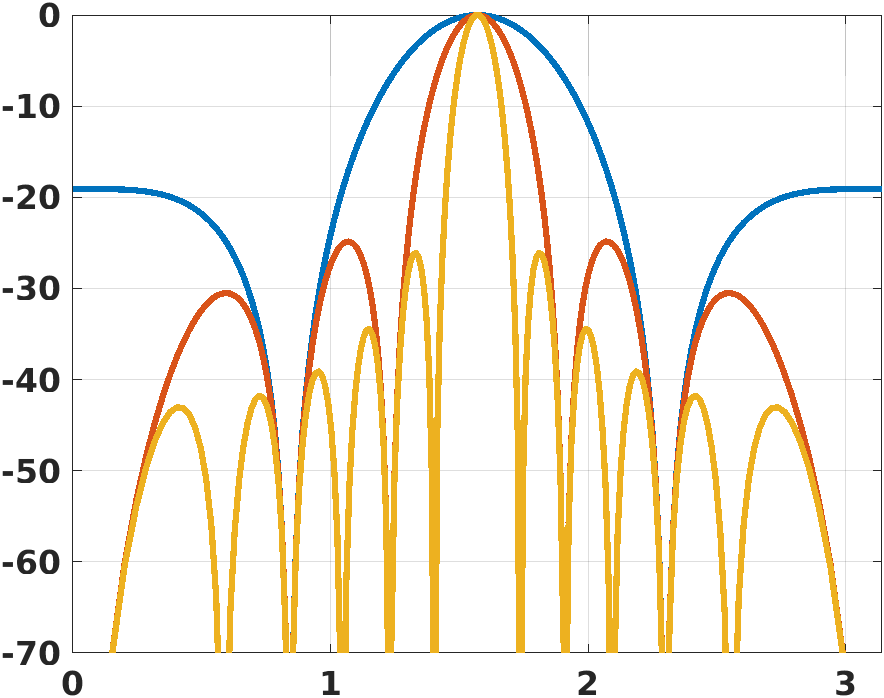
\includegraphics[width=\linewidth]{./Media/fig_commonBp_1.png}
    \begin{overpic}[width=\linewidth, 
        %grid, 
        tics=10,trim=0 0 0 0]{./Media/fig_commonBp_1.png}
            \put (19, 58){\tiny{$N\!=\!3$}}
            \put (19, 47){\tiny{$N\!=\!6$}}
            \put (19, 34){\tiny{$N\!=\!12$}}
    \end{overpic}
    \caption{}
    \label{fig_common_bps1}
  \end{subfigure}
  %
  \begin{subfigure}[b]{0.4\linewidth}
    \begin{overpic}[width=\linewidth, 
        %grid, 
        tics=10,trim=0 0 0 0]{./Media/fig_commonBp_2.png}
            \put (81, 63.5){\tiny{$N\!=\!3$}}
            \put (76, 57){\tiny{$N\!=\!6$}}
            \put (76, 53){\tiny{$N\!=\!12$}}
    \end{overpic}
    \caption{}
    \label{fig_common_bps2}
  \end{subfigure}
  \caption{Two common ways of visualizing the array's response in the 2D planar case.
  In both plots, a comparison between the CB's responses of 3,6 and 12 elements arrays is simulated. 
  In Fig.~\ref{fig_common_bps1}, the response is presented on the $\vBrace{0,\pi}$ interval with units of dB.
  In Fig.~\ref{fig_common_bps2}, a polar plot is presented with same units for the response gain but the DOA is in degrees.}
  \label{fig_common_bps}
\end{figure}
For sensors in 3D space the DOA depends on two angles (azimuth and elevation).
However, for the sake of simplicity, we consider a planar (i.e. azimuth without elevation) DOA such that the beampattern is a function of an angle $\theta$
\begin{equation}
B\rBrace{\theta} = \abs{Z\rBrace{\theta}}.
\end{equation}
The beampttern is commonly presented in a graphical manner with log scale as exemplified in Fig.~\ref{fig_common_bps}.
It's characteristics, such as main lobe width, position and attenuation of sidelobes are then analysed and compared between different schemes.
The analysis can be done theoretically, when the beampattern's mathematical expression is known or it can be conducted numerically.
% In this work, as we deal with 2D planar localization problems, we find the presentation of Fig.~\ref{fig_common_bps1} most suitable.
The DOAs of the impinging signal may be presented in various ways where units may be degrees or radians.
% Also, as the DOA is periodical one should also choose the centering, for example when the beampattern is steered towards different angles and the author wants to center the mainlobe.
In this work, we choose to follow \cite{van2004optimum}'s $\psi$-space, i.e.
\begin{equation}
    \psi\rBrace{\theta_{d}}=\frac{2\pi}{\lambda}\cos{\theta_{d}}\cdot{}d,
\end{equation}
where $\lambda$ is the impinging signal's wavelength.
% The reader may notice that $\psi$ is exactly the electric phase $\theta$ defined in \eqref{eq:thetaULA} therefore, throughout the rest of the work, we use the $\theta$ notation. 
% Also, we choose to plot beampatterns using $\Delta\theta = \theta\rBrace{\theta_{d}} - \theta\rBrace{\theta_{s}}$, where $\theta_{s}$ is the steering angle of the array, it centers the mainlobe, enabling convenient comparison.
\subsection{The normalized beampattern}
As the absolute output gain is system dependent, comparing two different beampatterns is not possible where their maximal gain of the mainlobe are different.
Therefore, a common practice \cite{van2004optimum} when analysing the array's spatial performance, is to normalize the beampattern such that the mainlobe's output gain at it's peak is 1 (0dB), thus enabling convenient comparable measures extraction.
This quantity will be referred to as $$\mathcal{H}\rBrace{\theta} = H\rBrace{\theta}/H\rBrace{\theta_{s}}$$ where $H$ is the array's response and $\theta_{s}$ is the DOA that the array is steered to.
\subsection{Half power beamwidth}
% Considering localization problems, possibly the main interest is spatial resolution, related to localization accuracy and distinction of spatially close objects, where ``close`` can be interpreted as small physical distance between objects of interest or objects that may be physically distant from each other but from the array's perspective are in relatively similar.
% \par
Considering localization problems, the spatial resolution is obviously linked to the main lobe's width, i.e. higher resolution is achieved for narrower main lobe.
The Half Power BeamWidth (HPBW), marked as $\Delta\theta_{HPBW}$, is defined to be the 3-dB beamwidth, i.e. the point where $\abs{B\rBrace{\theta}}^{2} = 0.5$ or $\abs{B\rBrace{\theta}} = 1/\sqrt{2}$.
For standard $N$-element ULA, assuming large $N$ values, it is known \cite{van2004optimum} that
\begin{equation}
    \label{eq_known_HBPW}
    \dThetaHPBW/2= 1.4/N.
\end{equation}
\par
Obviously, we aim to show that the presented architecture increases the resolution, compared to other arrays by proving that the beamwidth shrinks below the $1.4/N$ limit.
%
%
%
\subsection{Sidelobes attenuation}
% As the beampattern consists of multiple harmonics (as the number of elements $N$), sidelobes occur when the some harmonics are summed, showing as peaks other than the mainlobe.
% As this is an unwanted result, the height and their rate of decrease are measured aiming to prefer arrays where their height is reduced and the decrease rate is increased.
A known \cite{van2004optimum} parasitic phenomenon of beampatterns is sidelobes, which manifests as energy peaks outside the mainlobe, typically highest near the mainlobe and decreasing towards the edges of the beampattern.
In the context of localization, this can cause false detection or reduction in spatial resolution.
Related spatial performance metrics are the sidelobes gain and rate of decrease in sidelobe gain.
%
%
%
\subsection{Directivity}
A common measure of performance of an array or aperture is the directivity $\mathcal{D}$.
As in \cite{van2004optimum}, in a transmitting array, $\mathcal{D}$ represents the maximum radiation intensity (power per DOA) divided by the average radiation intensity (averaged over all DOAs).
Also, in a receiving array, the denominator represents the noise power at the array output due to isotropic noise (noise distributed uniformly over all DOAs). 
The numerator will represent the power due to a signal arriving from a certain DOA ($\theta_{d}$) - Thus, $\mathcal{D}$ can be interpreted as the array gain against isotropic noise.
We define the power pattern, $P\rBrace{\theta_{d}}$, to be the squared magnitude of the beampattern $B\rBrace{\theta_{d}}$
\begin{equation}
    P\rBrace{\theta_{d}} = \abs{B\rBrace{\theta_{d}}}^{2}
\end{equation}
where the frequency dependence is suppressed.
Then the directivity $\mathcal{D}$ is defined as
\begin{equation}\label{eq_D}
    \mathcal{D}\rBrace{\theta_{d}} = \frac{
    P\rBrace{\theta_{d}}
    }{
    \frac{1}{2\pi}\int_{0}^{2\pi}P\rBrace{\theta}d\theta
    }.
\end{equation}
% In the following, as we consider steered (to $\theta_{s}$) arrays, we suppress the DOA dependency such that $\mathcal{D} = \mathcal{D}\rBrace{{\theta_{s}}}$. 
and for uniformly weighted ULAs, it is known \cite{van2004optimum} that $\mathcal{D} = N$.
